%!TEX program = xelatex
\documentclass[tikz]{standalone}
\usepackage{ctex}
\usepackage{fontawesome}
\usepackage{tikz}
\usepackage{epstopdf}
\usetikzlibrary{arrows,decorations.markings}
\definecolor{bubbles}{rgb}{0.91, 1.0, 1.0}
\definecolor{shadow}{rgb}{0.54, 0.47, 0.36}

\begin{document}
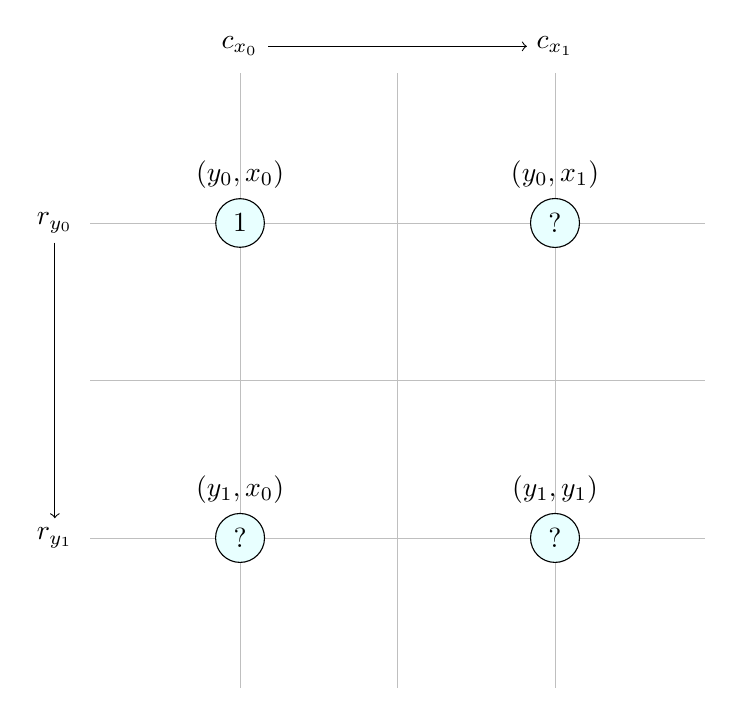
\begin{tikzpicture}[decoration={
    markings,
    mark=at position 1 with {\arrow[scale=1]{angle 90}};
  }]
  \draw[opacity=.5,help lines,step=2] (0.1,0.1) grid (7.9,7.9);
  \node[circle,draw,fill=bubbles,minimum size=0.5cm,label=above:{$(y_0,x_0)$}] at (2,6) {$1$};
    \node[circle,draw,fill=bubbles,minimum size=0.5cm,label=above:{$(y_0,x_1)$}] at (6,6) {?};
    \node[circle,draw,fill=bubbles,minimum size=0.5cm,label=above:{$(y_1,x_0)$}] at (2,2) {?};
    \node[circle,draw,fill=bubbles,minimum size=0.5cm,label=above:{$(y_1,y_1)$}] at (6,2) {?};
    \node[left] (r1) at (0,6) {${r_{y_0}}$};
    \node[left] (r2) at (0,2) {${r_{y_1}}$};
    \node[above] (c1) at (2,8) {${c_{x_0}}$};
    \node[above] (c2) at (6,8) {${c_{x_1}}$};
    \draw[->] (r1) -- (r2);
    \draw[->] (c1) -- (c2);
\end{tikzpicture}

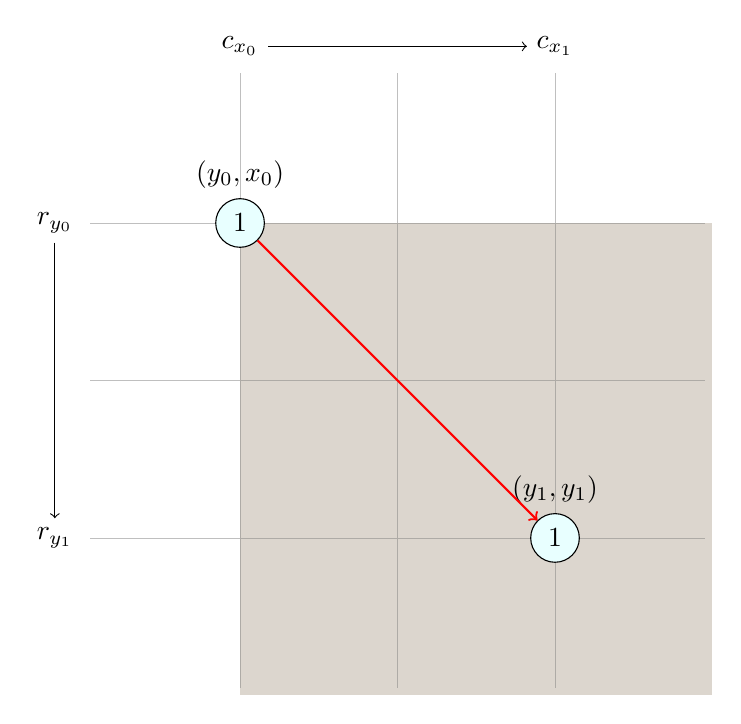
\begin{tikzpicture}[decoration={
    markings,
    mark=at position 1 with {\arrow[scale=1]{angle 90}};
  }]
  \fill[opacity=.3,color=shadow] (2,6) rectangle (8,0);
  \draw[opacity=.5,help lines,step=2] (0.1,0.1) grid (7.9,7.9);
  \node[circle,draw,fill=bubbles,minimum size=0.5cm,label=above:{$(y_0,x_0)$}] (start) at (2,6) {$1$};
  \node[circle,draw,fill=bubbles,minimum size=0.5cm,label=above:{$(y_1,y_1)$}] (end) at (6,2) {$ 1$};
    \node[left] (r1) at (0,6) {${r_{y_0}}$};
    \node[left] (r2) at (0,2) {${r_{y_1}}$};
    \node[above] (c1) at (2,8) {${c_{x_0}}$};
    \node[above] (c2) at (6,8) {${c_{x_1}}$};
    \draw[->] (r1) -- (r2);
    \draw[->] (c1) -- (c2);
    \draw[->,red,thick] (start) -- (end);
\end{tikzpicture}

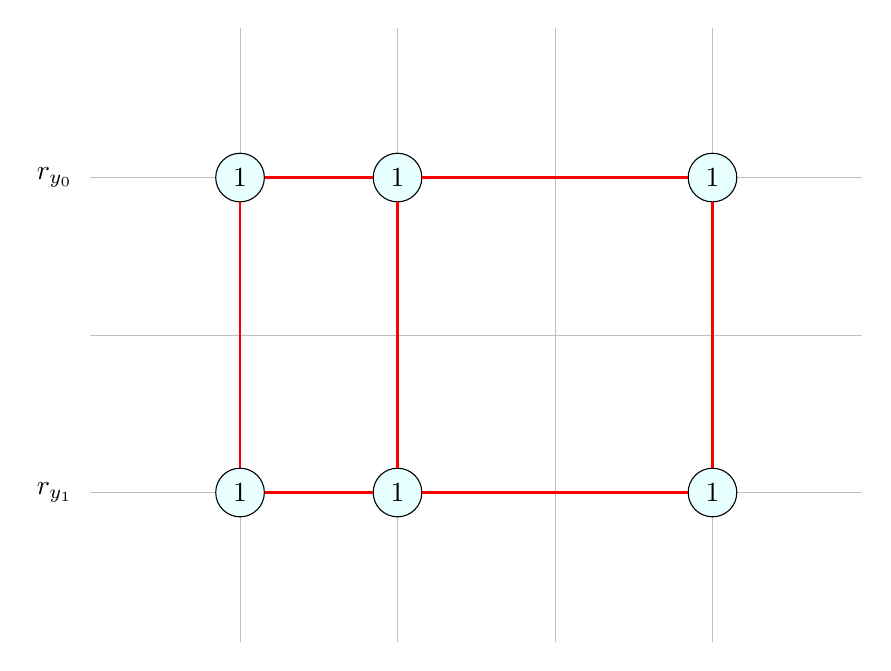
\begin{tikzpicture}[decoration={
    markings,
    mark=at position 1 with {\arrow[scale=1]{angle 90}};
  }]
  \draw[opacity=.5,help lines,step=2] (0.1,0.1) grid (9.9,7.9);
  \node[circle,draw,fill=bubbles,minimum size=0.5cm] (x1) at (2,6) {$1$};
  \node[circle,draw,fill=bubbles,minimum size=0.5cm] (x2) at (4,6) {$1$};
  \node[circle,draw,fill=bubbles,minimum size=0.5cm] (x3) at (8,6) {$1$};
  \node[circle,draw,fill=bubbles,minimum size=0.5cm] (y1) at (2,2) {$1$};
  \node[circle,draw,fill=bubbles,minimum size=0.5cm] (y2) at (4,2) {$1$};
  \node[circle,draw,fill=bubbles,minimum size=0.5cm] (y3) at (8,2) {$1$};
    \node[left] (r1) at (0,6) {${r_{y_0}}$};
    \node[left] (r2) at (0,2) {${r_{y_1}}$};
    \draw[red,thick] (x1) -- (y1);
    \draw[red,thick] (x2) -- (y2);
    \draw[red,thick] (x3) -- (y3);
    \draw[red,thick] (x1) -- (x2);
    \draw[red,thick] (x2) -- (x3);
    \draw[red,thick] (y1) -- (y2);
    \draw[red,thick] (y2) -- (y3);
\end{tikzpicture}
\end{document}
